\section{MODULO: SISTEMA DE CONTROL DIFUSO}

\subsection{Simulación de la planificación de movimiento}

Como se mencionó anteriormente el problema se puede clasificar dentro de los de planificación de movimiento (motion planning), se debe mover un objeto (robot) desde un punto inicial a un punto final evitando colisionar con los posibles obstáculos del entorno. El robot conoce su pose (el ángulo hacia dónde se orienta respecto al eje de coordenadas) en todo momento y el ángulo hacia el target, además no presenta limitaciones en cuanto al ángulo de giro. La detección de obstáculos se realiza mediante tres sensores de distancia.

Algunas consideraciones que se tuvieron en cuenta para el armado de reglas y funciones de pertenencia [6].

\begin{itemize}
    \item Cubrir adecuadamente el espacio de estado del problema.
    \item El conjunto de reglas debe ser completo y correcto.
    \item Las reglas no deben ser contradictorias.
    \item Para todos los valores de entrada la suma del grado de pertenencia de los distintos conjuntos debe ser 1.
\end{itemize}

\subsubsection{Módulos de control propuestos}

El desarrollo de la solución se puede dividir en versiones que van desde menor a mayor complejidad. Partiendo de un ejemplo de simulación y control difuso implementado en matlab que muestra como ajustar un sistema de lógica difusa usando una función de costo personalizada y que se puede encontrar \href{https://www.mathworks.com/help/fuzzy/tune-fuzzy-systems-using-custom-cost-function.html}{\textbf{aqui}}, a partir de ahora llamado "MySimAvoidObs1".

\paragraph{MySimAvoidObs1}\mbox{}\\

Nuestra idea base, fue controlar con el sistema difuso la variación del ángulo actual del robot para evadir un obstáculo. En este planteo el robot no tiene información sobre el destino, solo se encarga de evadir obstáculos. De este modo se representa el control con el siguiente esquema.

\subparagraph{Variables MySimAvoidObs1}\mbox{}\\


\paragraph{MySimAvoidObs2}\mbox{}\\

\begin{center}
    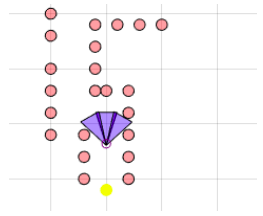
\includegraphics[scale=0.5]{Tesis/Capitulos/04_CAPITULO_2/img/des1.png}
    \captionof{figure}{Captura de la simulacion de MySimAvoidObs2.}
\end{center}

\begin{center}
    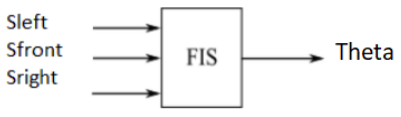
\includegraphics[scale=0.5]{Tesis/Capitulos/04_CAPITULO_2/img/esquema1.png}
    \captionof{figure}{Esquema de entradas y salidas MySimAvoidObs2.}
\end{center}

En donde Sleft, Sfront, y Sright representa las distancias al obstáculo y Theta el ángulo que deberá girar el robot para evadirlo.

\subparagraph{Variables MySimAvoidObs2}\mbox{}\\

A continuación se muestra el detalle de las funciones de pertenencia de las variables intervinientes en el control difuso. Consideramos como entradas la distancia al obstáculo obtenida mediante tres sensores con ángulo ajustable. En los tres sensores se repiten las funciones “cerca” y “lejos”.